\documentclass[../AnalysisNoteJBuxton.tex]{subfiles}
\begin{document}

\subsection{Model: Lambda-Kaon}
\label{ModelLambdaKaon}

Talk about Lednicky model

\begin{equation}
\begin{array}{l}
\vspace{2mm}  %%space between C(k^{*}) and C_{FSI}(k^{*})
  C(k^{*}) = 1+\lambda[\alpha\exp(-4k^{*2}R^{2})+C_{FSI}(k^{*})] \\
\vspace{2mm}  %%space between C_{FSI}(k^{*}) and f(k^{*})
  C_{FSI}(k^{*}) = (1+\alpha)[\frac{1}{2}|\frac{f(k^{*})}{R}|^2(1-\frac{d_{0}}{2\sqrt{\pi}R})+\frac{2\mathbb{R}f(k^{*})}{\sqrt{\pi}R}F_{1}(2k^{*}R)-\frac{\mathbb{I}f(k^{*})}{R}F_{2}(2k^{*}R)] \\
\vspace{2mm}  %%space after f(k^{*})  
  f(k^{*}) = (\frac{1}{f_{0}}+\frac{1}{2}d_{0}k^{*2}-ik^{*})^{-1}
\end{array}  
\label{eqn:LednickyEqn}
\end{equation}

\begin{figure}[h]
  \centering
  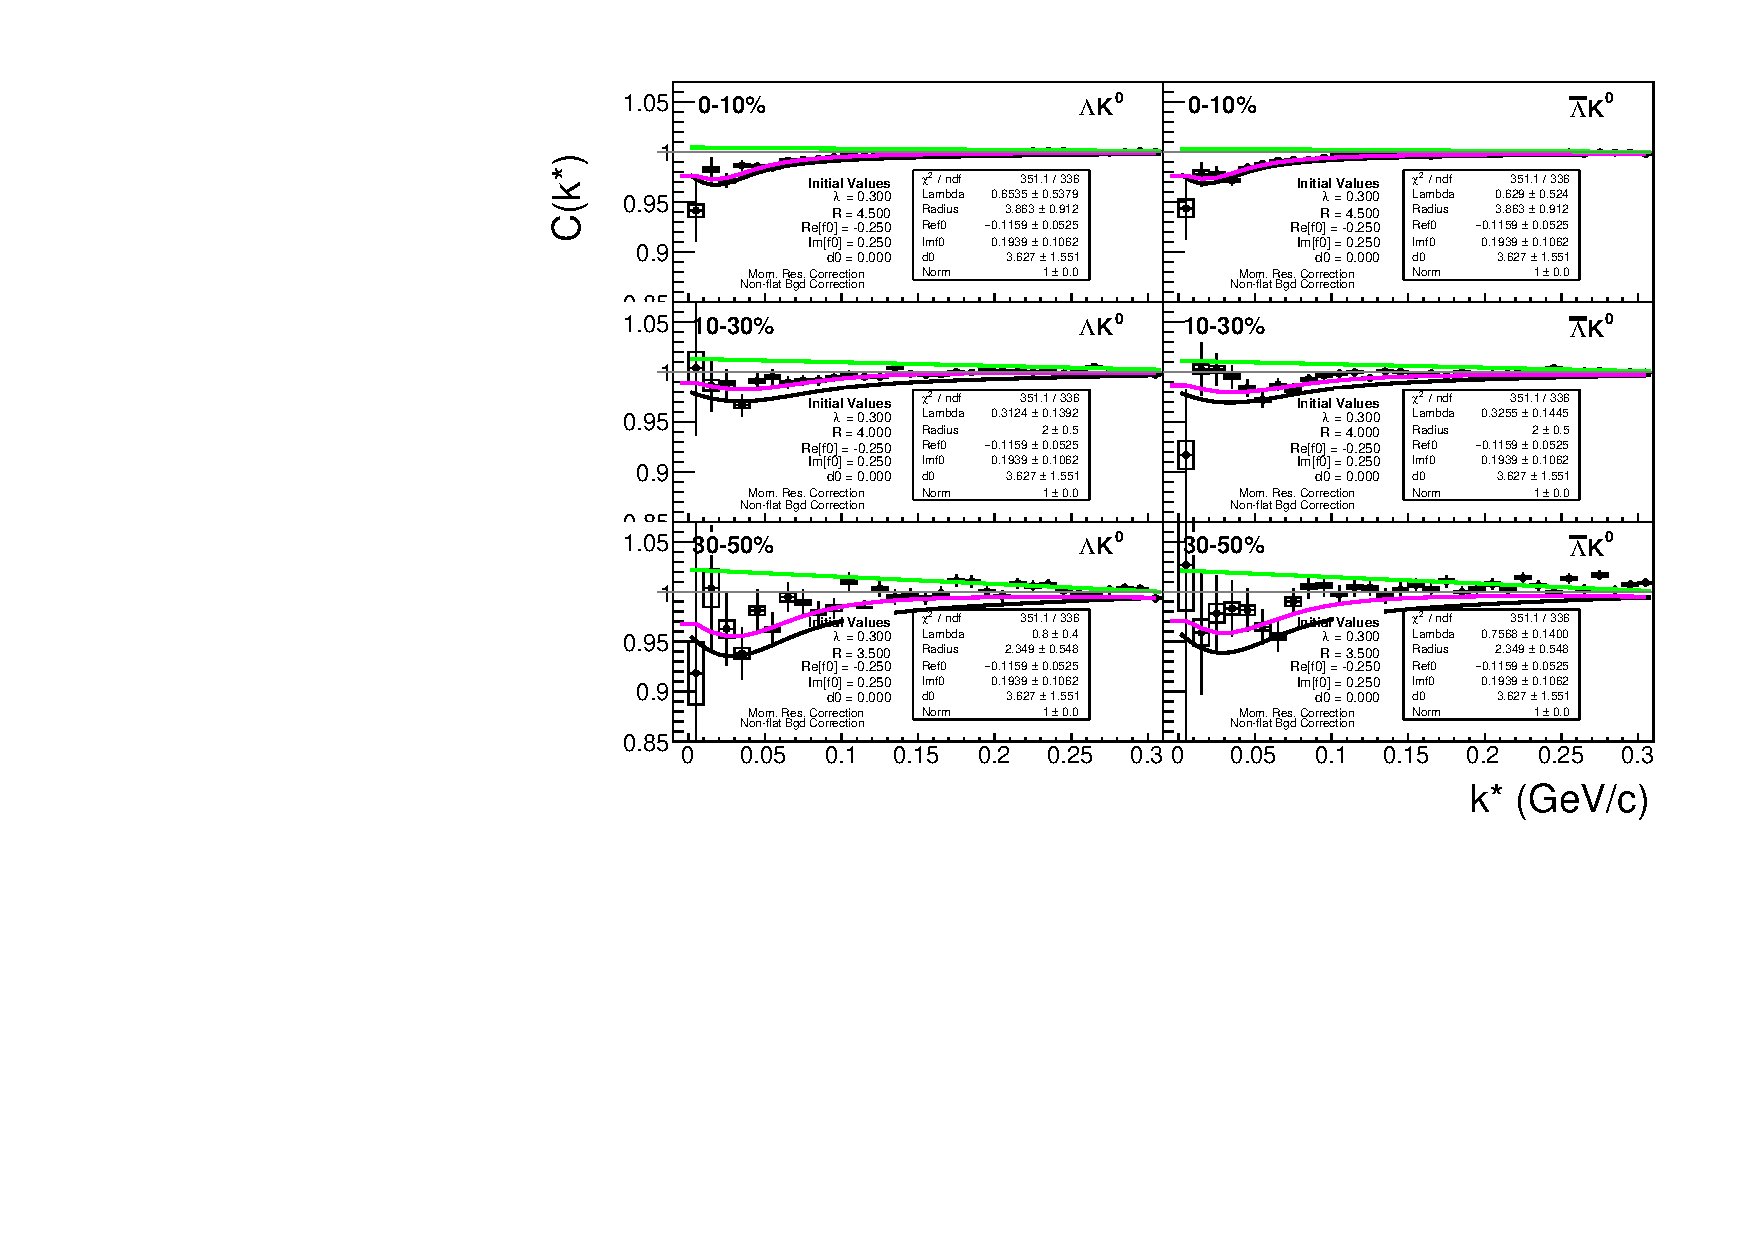
\includegraphics[width=\textwidth]{5_Fitting/Figures/canKStarCfwFitsLamK0wConj_MomResCrctn_NonFlatBgdCrctn.pdf}
  \caption[$\Lambda$K$^{0}_{S}$($\bar{\Lambda}$K$^{0}_{S}$) Fits]{$\Lambda$K$^{0}_{S}$($\bar{\Lambda}$K$^{0}_{S}$) Fits}
  \label{fig:LamK0wConjFits}
\end{figure}


\begin{figure}[h]
  \centering
  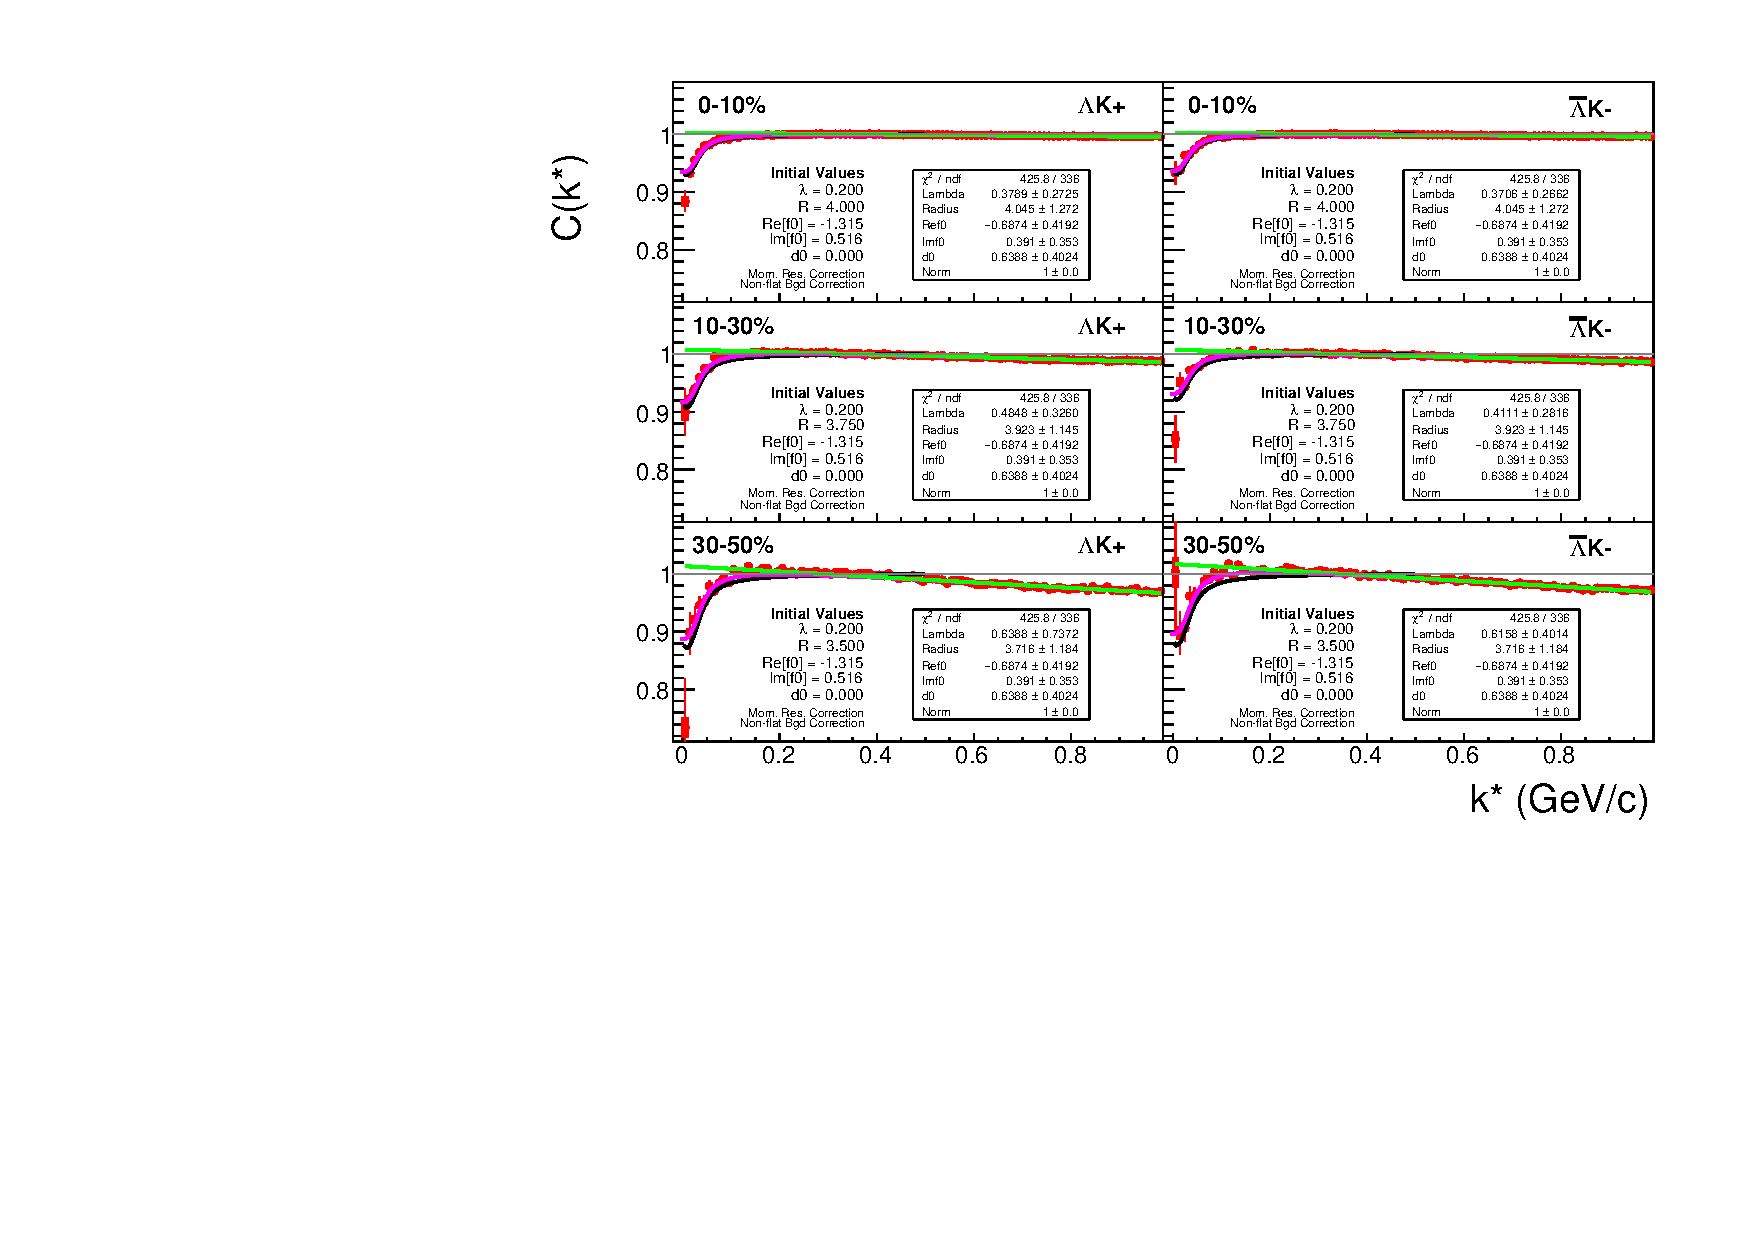
\includegraphics[width=\textwidth]{5_Fitting/Figures/canKStarCfwFitsLamKchPwConj_MomResCrctn_NonFlatBgdCrctn.pdf}
  \caption[$\Lambda$K$^{+}$($\bar{\Lambda}$K$^{-}$) Fits]{$\Lambda$K$^{+}$($\bar{\Lambda}$K$^{-}$) Fits}
  \label{fig:LamKchPwConjFits}
\end{figure}

\begin{figure}[h]
  \centering
  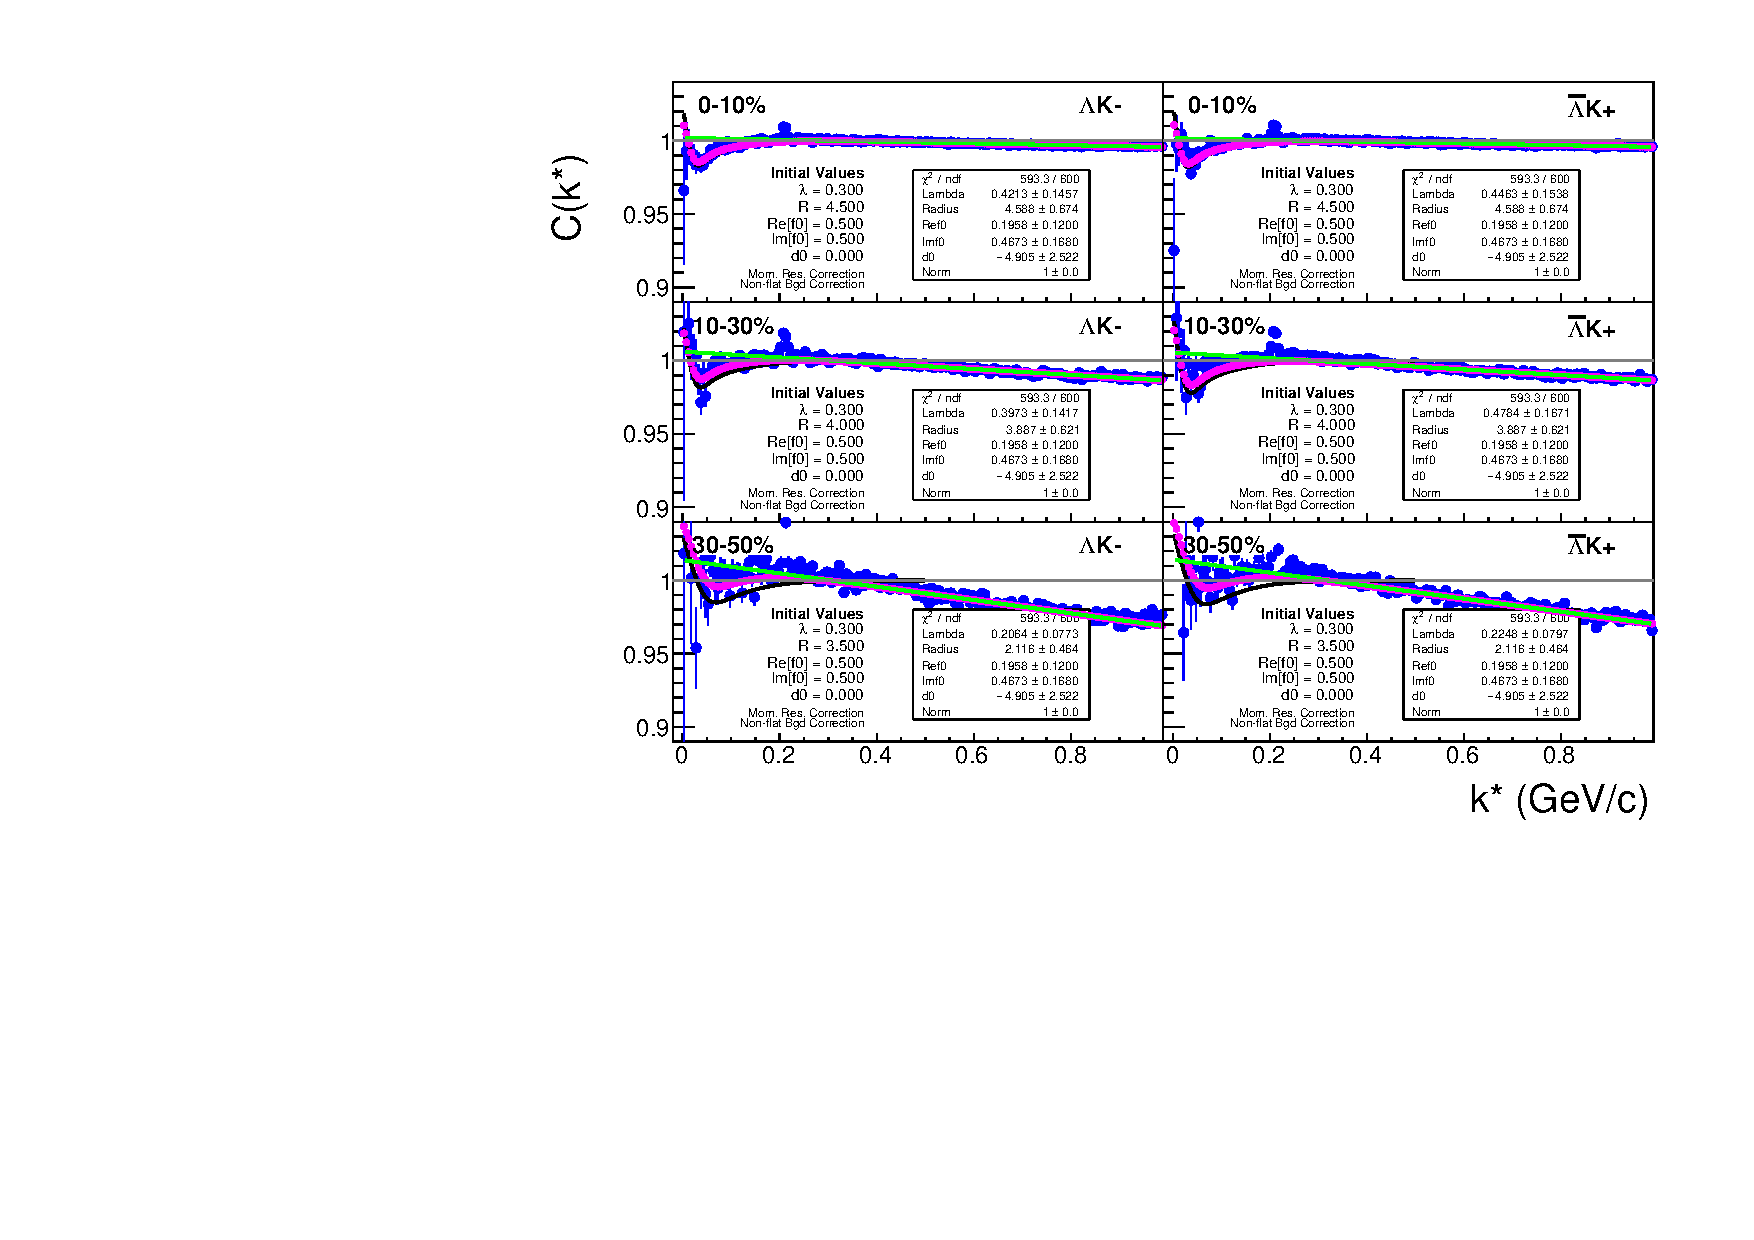
\includegraphics[width=\textwidth]{5_Fitting/Figures/canKStarCfwFitsLamKchMwConj_MomResCrctn_NonFlatBgdCrctn.pdf}
  \caption[$\Lambda$K$^{-}$($\bar{\Lambda}$K$^{+}$) Fits]{$\Lambda$K$^{-}$($\bar{\Lambda}$K$^{+}$) Fits}
  \label{fig:LamKchMwConjFits}
\end{figure}

\end{document}